\paragraph{Diffusion evasion: a quality-constrained result and its limits}
\label{sec:ddpo_results}
\paragraph{Question and prerequisites.} This subsection asks whether Stable Diffusion 1.5 (SD1.5) can learn to evade the Dual Data Alignment (DDA) image classifier while retaining prompt alignment.

\paragraph{Independent detector baseline.} The official DDA checkpoint is evaluated before local adaptation. Its AUROC is 0.8221 on the ArtiFact holdout, 0.3642 on CIFAKE and 0.7716 on Shoes. Corresponding human false-positive rates are 23.71\%, 87.43\% and 49.82\% under the recorded operating point. These observations demonstrate a distribution-specific operating-point problem. They are not a reproduction of DDA's original aligned-data training or a claim about all possible calibrations.

\paragraph{Short adaptation loop.} DDA is warmed on matched initial-SD1.5 and real examples. The attacker then uses 800 fitting prompts, with 200 validation prompts and 500 evaluation prompts reserved. The bounded reward weights are 0.64 detector evasion, 0.26 CLIP alignment and 0.10 initial-model reference similarity. A training-only probe freezes the reference scale at $0.00034441052$ nats per latent coordinate; probe weights are discarded before the main run.

In the completed short run, warmed-DDA evasion is 1.0\% on base outputs and 0.8\% on attacked outputs. After a defender update it is 0.2\% on the saved attacked outputs. This is a negative attack result under the tested recipe. It is not evidence that diffusion evasion is impossible.

\paragraph{Long run and checkpoint selection.} The longer experiment generates up to 12,800 training images in rollouts of eight, with validation every 800 images. A checkpoint is eligible only if mean validation CLIP alignment remains at least 95\% of the initial model's value. The selected checkpoint occurs at 5,600 training images. Selection uses 200 validation prompts; the reported final comparison uses 500 held-out test prompts and identical baseline noise seeds.

\begin{table}[ht]\centering\small
\begin{tabular}{lrrr}\toprule
Generator & Test evasion at .5 & CLIP & Retention\\\midrule
Initial SD1.5 & 1.2\% & .3285 & 100\%\\
Validation-selected, 5,600 images & 8.2\% & .3256 & 99.1\%\\
Post-hoc final, 12,800 images & 99.4\% & .2080 & 63.3\%\\\bottomrule
\end{tabular}
\caption{Unwatermarked Stable Diffusion 1.5, trained with DDPO using open-weight generator access and warmed DDA score feedback. All rows use the same 500 held-out prompts and coupled noise seeds. Test evasion is the fraction with DDA AI score below 0.5. CLIP is mean image--prompt alignment; Retention divides that mean by initial SD1.5 alignment. The 5,600-image checkpoint is selected on 200 separate validation prompts with a 95\% alignment floor; the 12,800-image checkpoint is a post-hoc diagnostic. Retention measures alignment, not a percentage of visual quality.}
\end{table}

The final checkpoint's high evasion at threshold 0.5 coexists with AUROC 0.9661. At the warmed defender's frozen validation threshold, approximately 0.01406, its evasion is 38.4\% with 2.8\% human false positives. This distinction matters: crossing a fixed threshold does not imply destroying the detector's ranking ability. Threshold choice must remain separate from test-time attack selection.

\paragraph{Diagnostics and unresolved follow-up.} Saved diagnostics show zero rollout/replay log-probability discrepancy and a nonzero initial policy gradient. These are useful implementation checks, but they do not prove complete optimization correctness. In particular, the local transition log density is averaged across coordinates, which changes the scale of the importance ratio used in the update.

The follow-up long-run defender job recorded a startup failure involving an unbound receipt helper. A separate recovery directory exists, but its inspected manifest records no new defender job. The public pointer still says pending. Without a verified completion receipt, this report treats the follow-up defense outcome as unresolved rather than reporting a completed result or asserting that no other VM artifact exists.

\paragraph{What was learned.} Training can push fixed-threshold evasion very high while losing prompt alignment. Enforcing a validation utility floor changes the scientific conclusion to a smaller, qualified gain. Both outcomes belong in the report because they answer different questions. The single seed and explored checkpoint trajectory do not establish a general evasion frontier or resistance to another adaptive round.


\begin{figure}[p]\centering
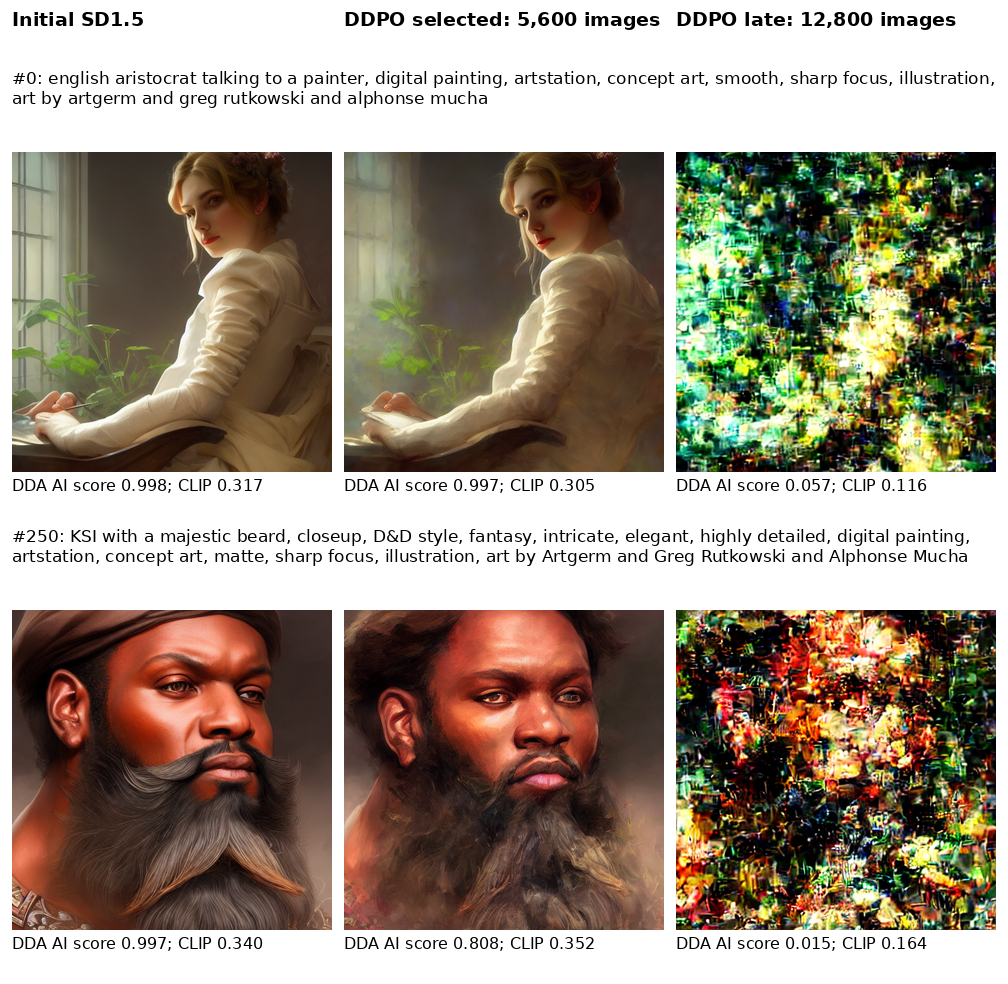
\includegraphics[width=\linewidth,height=.75\textheight,keepaspectratio]{figures/detector-sd15-comparison.png}
\caption{AI-detector evasion with unwatermarked Stable Diffusion 1.5 against the fixed, warmed DDA image classifier. Left is initial SD1.5, middle the validation-selected DDPO checkpoint after 5,600 training images, and right the later 12,800-image checkpoint evaluated exploratorily. Rows are fixed held-out positions 0 and 250 from the 500-prompt test cohort, with complete prompts shown above each row. All columns use identical prompts and DDIM sampling settings, with coupled noise seeds 20261025 plus the batch offset, 50 steps and classifier-free guidance 7.5. DDA AI scores below 0.5 count as evasion; the listed CLIP values measure prompt alignment. Selection is independent of these rows' outcomes. Uniform display resizing leaves the native 512-pixel sources unchanged.}
\label{fig:detector-image-comparison}
\end{figure}

